\normalfalse \difficiletrue \tdifficilefalse
\correctionfalse

%\UPSTIidClasse{11} % 11 sup, 12 spé
%\newcommand{\UPSTIidClasse}{12}

\exer{Barrière Sympact $\star\star$ \label{C1:05:14}}
\setcounter{numques}{0}
\UPSTIcompetence{B2-13}
\index{Compétence B2-13}
\index{Barrière Sympact}
\ifcorrection
\else
\textbf{Pas de corrigé pour cet exercice.}
\fi

\ifprof
\else
Soit le mécanisme suivant. On a $\vect{AC}=H\vect{j_0}$ et $\vect{CB}=R\vect{i_1}$. De plus, 
$H=\SI{120}{mm}$ et $R=\SI{40}{mm}$. 

\begin{center}
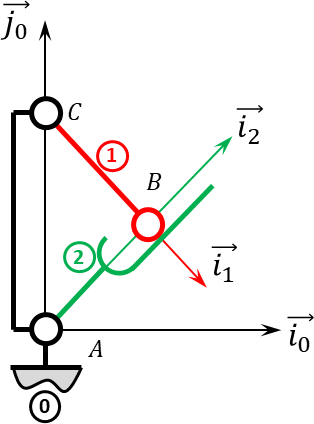
\includegraphics[width=\linewidth]{14_01}
\end{center}
\fi

On néglige la pesanteur sur la pièce \textbf{1}. 

On note $\torseurstat{\text{Moteur}}{1} = \torseurl{\vect{0}}{C_m\vk{0}}{\forall P}$ l'action mécanique du moteur sur la pièce \textbf{1}.

On note $\torseurstat{\text{Ressort}}{2} = \torseurl{\vect{0}}{C_r\vk{0}}{\forall P}$ l'action mécanique d'un ressort couple sur la pièce \textbf{2}. Le raideur du ressort est telle qu'il exerce un couple de \SI{45}{Nm} pour un angle de rotation 100\degres. On considère que le couple est nul lorsque la pièce 2 est à la verticale ($\varphi_o=\dfrac{\pi}{2}$). Il est au maximum lorsque $\varphi_f=0$.

On note $\torseurstat{\text{Pes}}{2} = \torseurl{-Mg\vj{0}}{\vect{0}}{\forall G}$ avec $\vect{AG}=L\vi{2}$. 

\question{Réaliser un graphe d'analyse.}
\ifprof
\else
\fi

\question{Expliciter $C_r$ en fonction des différents constantes ($k$, $\varphi_o$, $\varphi_f$) et celles qui vous sembleraient utile.}
\ifprof
\else
\fi

\question{Proposer une méthode permettant d'exprimer le couple moteur en fonction des autres actions mécaniques.}
\ifprof
\else
\fi


\ifprof
\else
\begin{flushright}
\footnotesize{Corrigé  voir \ref{C1:05:14}.}
\end{flushright}%
\fi